\section{Results: concentration with retained counterevidence}
\label{sec:results}

\paragraph{Classical structure and feasibility.}
Strict feasible retained states exist on 30/32 instances. Cluster repair improves over coordinate greedy on 25/32, with mean gain 17.019 (paired bootstrap CI [12.524,21.552]); collaboration rises descriptively from .475 to .664. These results justify a nontrivial classical control and show that workflow moves matter in the synthetic score. They do not establish superiority over mixed-integer programming, exhaustive full-instance optimization, or a broad ALNS portfolio. Moreover, only 27/32 cluster incumbents satisfy the composite feasibility predicate: five exceed review, service-scenario, or capacity-scenario tolerance, although all 32 have zero explicit disallowed-mode violations.

\paragraph{Conditional statevector signal.}
Mean exact optimum mass is .0223 under uniform retained-state sampling and .1522 under $p=2$ QAOA, a ratio of 6.831. The paired difference is .1299 with 95\% CI [.0991,.1640], and $p=2$ exceeds uniform on 30/32 instances. Under the frozen 128-draw simulations, mean first hit changes from 36.50 to 12.94; the paired difference is $-23.56$ draws [${-39.28},{-8.69}$]. Because a miss is coded as 129 and each method uses a single frozen draw sequence per instance, this is a matched sample-efficiency proxy rather than latency. The near-optimal coverage difference is +.0443 [${-.0208},.1120$], so its interval crosses zero and supports no clear coverage claim.

\begin{figure}[t]
  \centering
  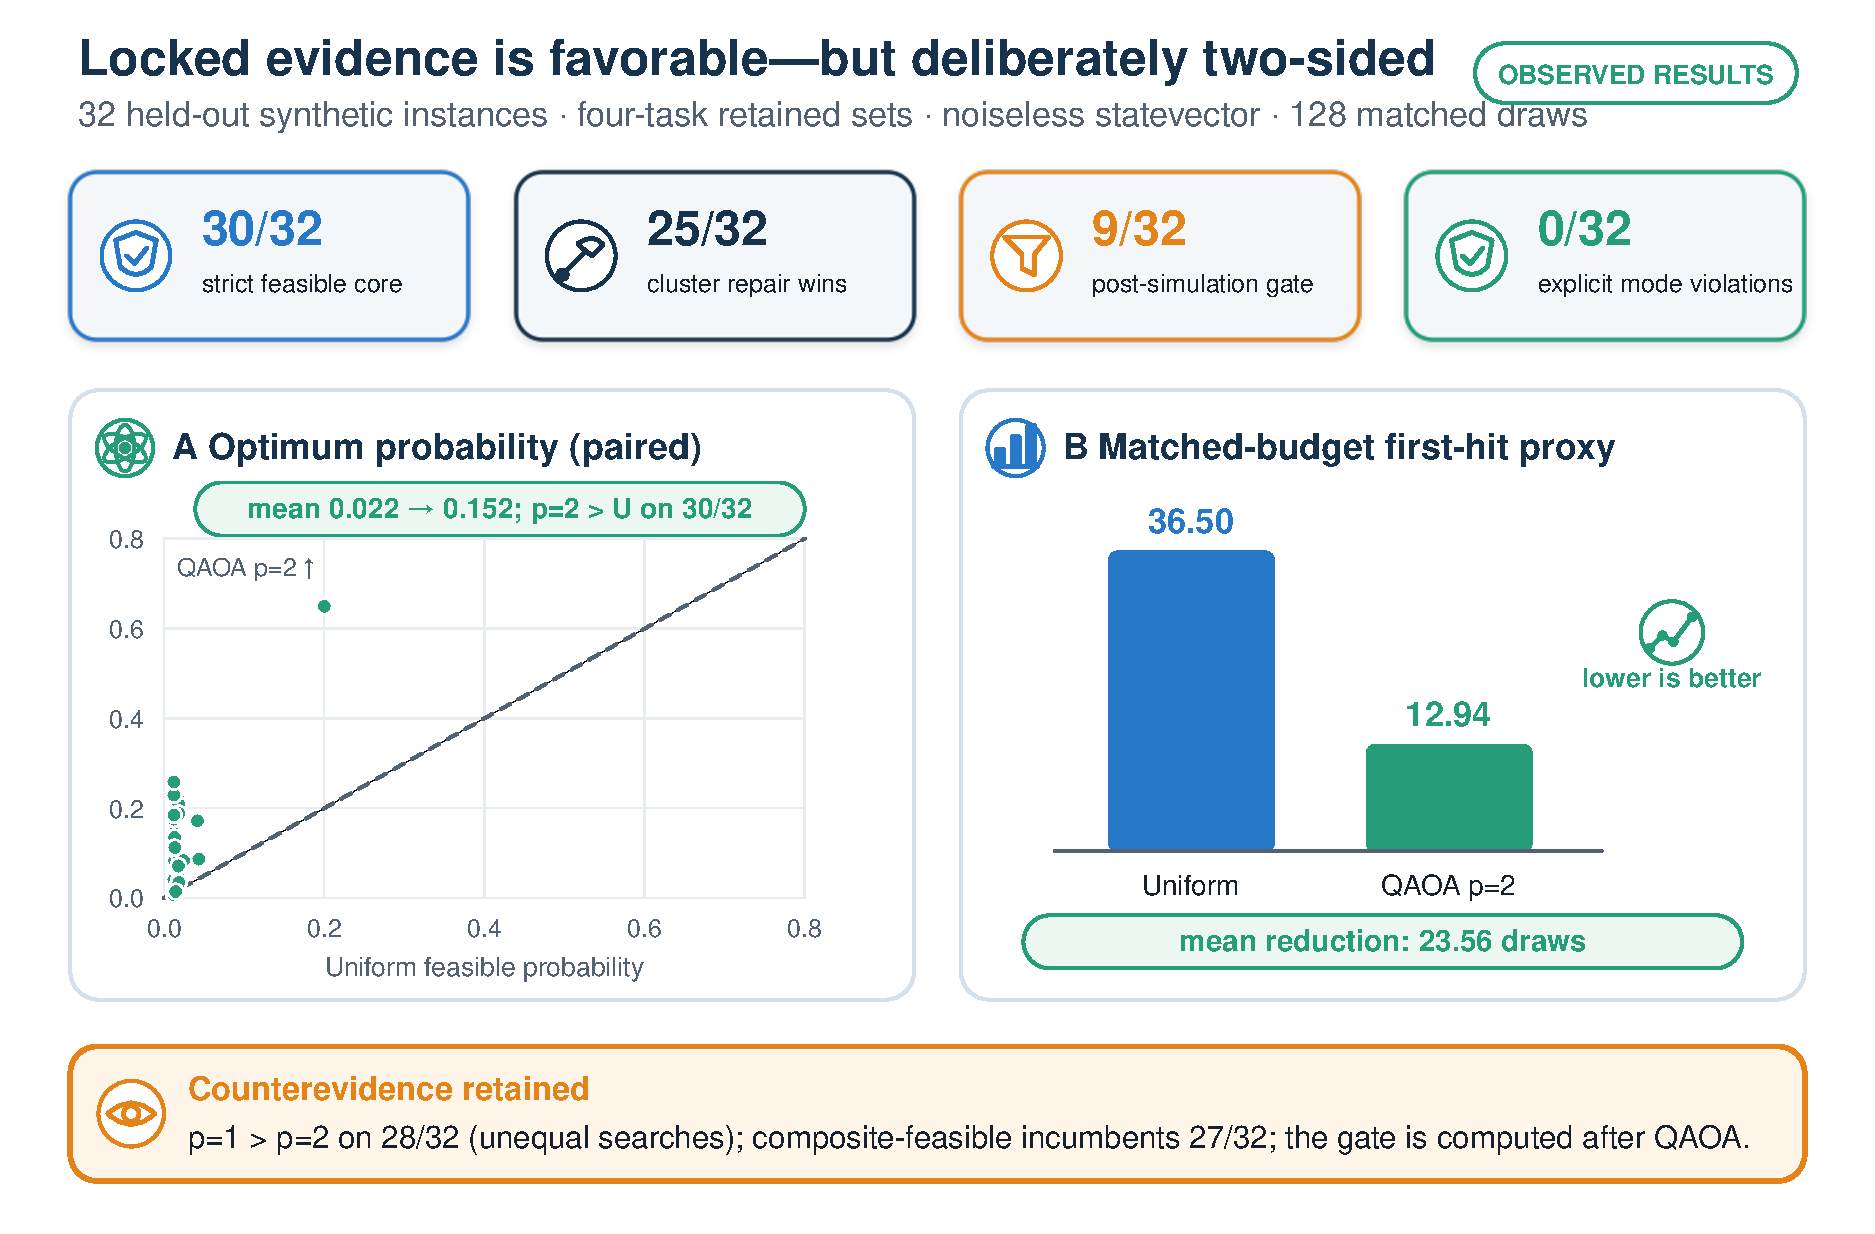
\includegraphics[width=\linewidth]{figs/fig5_results_dashboard.pdf}
  \caption{Frozen results. Panel A plots paired instance-level optimum masses; Panel B shows the matched-draw first-hit proxy. The orange strip preserves counterevidence needed to interpret depth, feasibility, and the post-simulation gate honestly.}
  \label{fig:results}
\end{figure}


\paragraph{Why ``selective'' remains an agenda, not a deployed policy.}
Only 9/32 cases satisfy the post-simulation gate. Ordered failures are 2 with no strict core, 7 with low classical ambiguity, and 14 with insufficient $p=2$ concentration. This partition is scientifically useful because it rejects a universal-use narrative. However, the gate observes the very quantum statistic whose computation a deployment router would decide whether to purchase. Calling it pre-execution ``adoption'' would therefore be target leakage. A credible invocation policy must learn or specify a decision from pre-simulation features and be frozen on separate instances.

\paragraph{Depth is counterevidence, not a success story.}
Mean $p=1$ optimum mass is .2492, and $p=1>p=2$ on 28/32 cases. Since $p=1$ receives 143 grid points while $p=2$ receives only 30 random candidates, neither circuit depth nor the parameter optimizer is isolated. The honest conclusion is that the frozen $p=2$ distribution concentrates probability relative to uniform, while deeper-is-better is unsupported. This pattern is consistent with the broader caution that variational performance depends on landscape, initialization and optimization budget~\citep{zhou2020qaoa,cerezo2021variational,blekos2024review}.

\begin{table}[t]
\centering
\caption{Reviewer-facing claim boundary.}
\label{tab:claims}
\scriptsize
\begin{tabularx}{\linewidth}{@{}p{0.21\linewidth}XX@{}}
\toprule
Risk & Defensible statement & Evidence still required \\
\midrule
``Quantum advantage'' & Conditional noiseless statevector concentration on frozen four-task retained sets. & QPU execution; wall-clock, energy and scaling comparisons. \\
``Selective invocation'' & A post-simulation evidence-eligibility gate partitions the frozen results. & A leakage-free pre-execution router evaluated out of sample. \\
``Zero violations'' & All incumbents have zero explicit disallowed-mode violations. & Composite feasibility holds for 27/32; deployment needs safety validation. \\
``Fair allocation'' & A regional AI-exposure dispersion regularizer is implemented. & Stakeholder-defined fairness constructs and disaggregated field outcomes. \\
``Depth helps'' & Both $p=1$ and $p=2$ were frozen and reported. & Equal-budget optimization, noise-aware sweeps and larger cores. \\
``First'' & Scoped review found no prior reproducible integration of all listed controls. & A systematic review could support a stronger priority claim. \\
\bottomrule
\end{tabularx}
\end{table}


\paragraph{Integrated significance.}
The benchmark contributes more than a QAOA toy by forcing the quantum comparison to inherit governance and stochastic feasibility from a shared evaluator. Conversely, the statevector result contributes less than a deployment demonstration: there is no QPU noise, transpilation, wall-clock or energy accounting, and the four-task retained space is exactly enumerable. The defensible result is a reproducible \emph{candidate concentration signal conditional on classical decomposition and certification}. Its value is methodological: it shows which controls, nulls and distinctions a future advantage claim must survive.
